\documentclass[12pt,a4paper]{article}
\usepackage[utf8]{vietnam}
\usepackage{amsmath,amssymb}
\usepackage{tabularx}
\usepackage{tikz}
\usepackage{xcolor}
\usepackage[top=0.6cm, bottom=0.6cm, left=0.6cm, right=0.6cm]{geometry}
\usepackage[dethi]{ex_test}

\SAOPTN{widthSA=2.6,heightSA=0.62}

\setlength{\parskip}{0pt}

% Dòng kẻ chấm mờ đều đặn chuẩn viết tay (khoảng cách 6.5mm rộng rãi vừa vặn)
\newcommand{\dongke}[1]{%
  \begingroup%
  \setlength{\parskip}{0pt}%
  \baselineskip=18.5pt%
  \vspace{1.0mm}%
  \foreach \i in {1,...,#1}{%
    \noindent{\color{gray!60}\dotfill}\par%
  }%
  \vspace{0.6mm}%
  \endgroup%
}

% Khu vực bài làm chia 2 cột có vách ngăn mờ ở giữa
\newcommand{\dongkeHaiCot}[1]{%
  \par\vspace{0.5mm}%
  \noindent%
  \begin{minipage}[t]{0.485\linewidth}%
    \dongke{#1}%
  \end{minipage}%
  \hfill%
  {\color{gray!60}\vrule}%
  \hfill%
  \begin{minipage}[t]{0.485\linewidth}%
    \dongke{#1}%
  \end{minipage}%
}

% Định nghĩa ô bài tập tự luận trong bảng
\newcommand{\oBaiTap}[3][5]{%
  \vspace{1.0mm}%
  \noindent\textbf{#2} #3\par%
  \dongke{#1}%
}

\begin{document}
\pagestyle{empty}
% =============================================================================
% ========================= TOÁN 7 - TUẦN 08 - BUỔI 01: MÃ ĐỀ 101 =============
% ========================= MẶT TRƯỚC (TRANG 1/2) ==============================
% =============================================================================

\noindent
\begin{tabularx}{\linewidth}{|X|c|}
\hline
\textbf{PHIẾU KIỂM TRA ĐỊNH KỲ TOÁN 7 - TUẦN 08 - BUỔI 01} & \textbf{Mã đề: 101 - Trang 1/2} \\
\hline
\end{tabularx}

\vspace{1.2mm}

\noindent
\begin{tabularx}{\linewidth}{|p{3.2cm}|X|}
\hline
\centering\textbf{ĐIỂM SỐ} & \centering\textbf{LỜI NHẬN XÉT CỦA THẦY CÔ} \tabularnewline
\hline
\rule{0pt}{1.8cm} & \tabularnewline
\hline
\end{tabularx}

\vspace{1.5mm}

\noindent\textbf{Câu 1 (0,25 điểm).} Số đối của số hữu tỉ $-\frac{5}{14}$ là: \shortans{\frac{5}{14}}\par\vspace{2.4mm}
\noindent\textbf{Câu 2 (0,25 điểm).} Giá trị của biểu thức $\sqrt{\frac{49}{100}}$ bằng: \shortans{\frac{7}{10}}\par\vspace{2.4mm}
\noindent\textbf{Câu 3 (0,25 điểm).} Giá trị của biểu thức $|-4{,}7| + |3{,}3|$ bằng: \shortans{8}\par\vspace{2.4mm}
\noindent\textbf{Câu 4 (0,25 điểm).} Làm tròn số thập phân $19{,}462$ đến hàng phần mười: \shortans{19{,}5}\par\vspace{2.4mm}
\noindent\textbf{Câu 5 (0,25 điểm).} Hai đường thẳng cắt nhau tạo góc $55^\circ$. Góc đối đỉnh với nó có số đo là: \shortans{55^\circ}\par\vspace{2.4mm}
\noindent\textbf{Câu 6 (0,25 điểm).} Cho hai góc kề bù $\widehat{xOy}$ và $\widehat{yOz}$, biết $\widehat{xOy} = 60^\circ$. Số đo $\widehat{yOz}$ là: \shortans{120^\circ}\par\vspace{2.4mm}
\noindent\textbf{Câu 7 (0,25 điểm).} Tia $Ot$ là tia phân giác của góc $\widehat{xOy} = 130^\circ$. Số đo của $\widehat{xOt}$ là: \shortans{65^\circ}\par\vspace{2.4mm}
\noindent\textbf{Câu 8 (0,25 điểm).} Cho $a \parallel b$. Một góc so le trong với góc $45^\circ$ có số đo là: \shortans{45^\circ}\par\vspace{2.4mm}
\noindent\textbf{Câu 9 (0,25 điểm).} Cho $a \parallel b$ và $c \perp a$. Quan hệ giữa hai đường thẳng $c$ và $b$ là: \shortans{\text{vuông góc}}\par\vspace{2.4mm}
\noindent\textbf{Câu 10 (0,25 điểm).} Một cặp sách giá $250\,000$ đ, giảm $20\%$. Số tiền được giảm là: \shortans{50\,000\text{ đ}}\par\vspace{2.4mm}
\vspace{0.4mm}

\noindent\textbf{Câu 11 (3,0 điểm). Thực hiện phép tính (hợp lý nếu có thể):}
\vspace{0.8mm}

\noindent
\begin{tabularx}{\linewidth}{|X|X|}
\hline
\oBaiTap[5]{a) (0,5 điểm)}{$\dfrac{7}{15} - \dfrac{5}{8} + \dfrac{8}{15} - \dfrac{3}{8}$} & 
\oBaiTap[5]{b) (0,5 điểm)}{$\dfrac{12}{19} \cdot \dfrac{5}{7} + \dfrac{12}{19} \cdot \dfrac{2}{7} - \dfrac{12}{19}$} \\
\hline
\oBaiTap[5]{c) (0,5 điểm)}{$\left(-\dfrac{1}{2}\right)^3 \cdot 16 + \left(\dfrac{2}{3}\right)^2 \cdot 9$} & 
\oBaiTap[5]{d) (0,5 điểm)}{$\sqrt{\dfrac{49}{16}} - \left|-\dfrac{3}{4}\right| + \sqrt{64}$} \\
\hline
\oBaiTap[5]{e) (0,5 điểm)}{$\left(\dfrac{3}{4} - 0{,}2\right) : \dfrac{11}{20} + \dfrac{5}{11} \cdot 1{,}1$} & 
\oBaiTap[5]{f) (0,5 điểm)}{$\dfrac{4^2 \cdot 9^3}{6^4}$} \\
\hline
\end{tabularx}

\newpage
% =============================================================================
% ========================= TOÁN 7 - TUẦN 08 - BUỔI 01: MÃ ĐỀ 101 =============
% ========================= MẶT SAU (TRANG 2/2) ================================
% =============================================================================

\noindent
\begin{tabularx}{\linewidth}{|X|c|}
\hline
\textbf{TOÁN 7 - TUẦN 08 - BUỔI 01} & \textbf{Mã đề: 101 - Trang 2/2} \\
\hline
\end{tabularx}

\vspace{1.5mm}

\noindent\textbf{Câu 12 (2,0 điểm). Tìm số hữu tỉ $x$, biết:}
\vspace{0.8mm}

\noindent
\begin{tabularx}{\linewidth}{|X|X|}
\hline
\oBaiTap[5]{a) (0,5 điểm)}{$x + \dfrac{2}{5} = \dfrac{9}{10}$} & 
\oBaiTap[5]{b) (0,5 điểm)}{$\dfrac{2}{3}x - \dfrac{1}{2} = \dfrac{5}{6}$} \\
\hline
\oBaiTap[5]{c) (0,5 điểm)}{$\left(x - \dfrac{1}{2}\right)^2 = \dfrac{9}{16}$} & 
\oBaiTap[5]{d) (0,5 điểm)}{$\left|2x - \dfrac{1}{3}\right| = \dfrac{5}{3}$} \\
\hline
\end{tabularx}

\vspace{1.5mm}

\noindent
\begin{tabularx}{\linewidth}{|X|}
\hline
\vspace{0.5mm}
\begin{minipage}[t]{0.68\linewidth}
\vspace{0pt}
\textbf{Câu 13 (2,0 điểm).} Cho hai tia $Ax$ và $By$ song song với nhau ($Ax \parallel By$). Điểm $O$ nằm giữa hai đường thẳng chứa tia $Ax$ và $By$ sao cho tia $Ax$ và tia $By$ cùng nằm về một phía đối với đường thẳng $AB$. Biết $\widehat{xAO} = 40^\circ$ và $\widehat{yBO} = 50^\circ$.\par\vspace{0.4mm}
\textbf{a) (1,0 điểm)} Kẻ tia $Oz \parallel Ax$ (tia $Oz$ nằm trong góc $\widehat{AOB}$). Giải thích vì sao $Oz \parallel By$.\par\vspace{0.4mm}
\textbf{b) (1,0 điểm)} Tính số đo góc $\widehat{AOB}$.
\end{minipage}\hfill
\begin{minipage}[t]{0.30\linewidth}
\vspace{0pt}\centering
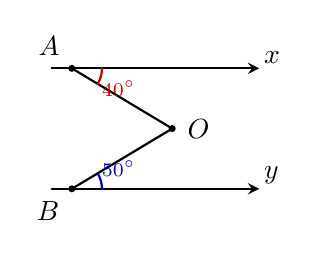
\begin{tikzpicture}[scale=0.85, >=stealth, line join=round, line cap=round]
  % Hai tia Ax va By
  \draw[thick, ->] (0.5, 2.3) -- (3.6, 2.3) node[above right=-2pt] {$x$};
  \draw[thick, ->] (0.5, 0.5) -- (3.6, 0.5) node[above right=-2pt] {$y$};
  
  % Doan AO va BO
  \draw[thick] (0.8, 2.3) -- (2.3, 1.4) -- (0.8, 0.5);
  
  % Diem A, B, O
  \fill (0.8, 2.3) circle (1.5pt) node[above left=1pt] {$A$};
  \fill (0.8, 0.5) circle (1.5pt) node[below left=1pt] {$B$};
  \fill (2.3, 1.4) circle (1.5pt) node[right=2pt] {$O$};
  
  % Goc xAO va yBO
  \draw[red!80!black, thick] (0.8, 2.3) ++(0:0.45) arc (0:-31:0.45);
  \node[red!80!black, font=\scriptsize] at (1.5, 2.0) {$40^\circ$};
  
  \draw[blue!80!black, thick] (0.8, 0.5) ++(0:0.45) arc (0:31:0.45);
  \node[blue!80!black, font=\scriptsize] at (1.5, 0.8) {$50^\circ$};
\end{tikzpicture}
\end{minipage}\par
\vspace{0.4mm}
\noindent\textit{Bài giải:}\dongkeHaiCot{10}
\\ \hline
\end{tabularx}

\vspace{1.5mm}

\noindent
\begin{tabularx}{\linewidth}{|X|}
\hline
\vspace{0.5mm}
\textbf{Câu 14 (0,5 điểm).} Tìm giá trị nhỏ nhất của biểu thức: $A = |x - 2026| + |x - 2|$.\par
\vspace{0.4mm}
\noindent\textit{Bài giải:}\dongkeHaiCot{6}
\\ \hline
\end{tabularx}

\newpage
% =============================================================================
% ========================= TOÁN 7 - TUẦN 08 - BUỔI 01: MÃ ĐỀ 102 =============
% ========================= MẶT TRƯỚC (TRANG 1/2) ==============================
% =============================================================================

\noindent
\begin{tabularx}{\linewidth}{|X|c|}
\hline
\textbf{PHIẾU KIỂM TRA ĐỊNH KỲ TOÁN 7 - TUẦN 08 - BUỔI 01} & \textbf{Mã đề: 102 - Trang 1/2} \\
\hline
\end{tabularx}

\vspace{1.2mm}

\noindent
\begin{tabularx}{\linewidth}{|p{3.2cm}|X|}
\hline
\centering\textbf{ĐIỂM SỐ} & \centering\textbf{LỜI NHẬN XÉT CỦA THẦY CÔ} \tabularnewline
\hline
\rule{0pt}{1.8cm} & \tabularnewline
\hline
\end{tabularx}

\vspace{1.5mm}

\noindent\textbf{Câu 1 (0,25 điểm).} Số đối của số hữu tỉ $-\frac{7}{18}$ là: \shortans{\frac{7}{18}}\par\vspace{2.4mm}
\noindent\textbf{Câu 2 (0,25 điểm).} Giá trị của biểu thức $\sqrt{\frac{64}{81}}$ bằng: \shortans{\frac{8}{9}}\par\vspace{2.4mm}
\noindent\textbf{Câu 3 (0,25 điểm).} Giá trị của biểu thức $|-5{,}6| + |3{,}4|$ bằng: \shortans{9}\par\vspace{2.4mm}
\noindent\textbf{Câu 4 (0,25 điểm).} Làm tròn số thập phân $28{,}371$ đến hàng phần mười: \shortans{28{,}4}\par\vspace{2.4mm}
\noindent\textbf{Câu 5 (0,25 điểm).} Hai đường thẳng cắt nhau tạo góc $65^\circ$. Góc đối đỉnh với nó có số đo là: \shortans{65^\circ}\par\vspace{2.4mm}
\noindent\textbf{Câu 6 (0,25 điểm).} Cho hai góc kề bù $\widehat{xOy}$ và $\widehat{yOz}$, biết $\widehat{xOy} = 70^\circ$. Số đo $\widehat{yOz}$ là: \shortans{110^\circ}\par\vspace{2.4mm}
\noindent\textbf{Câu 7 (0,25 điểm).} Tia $Ot$ là tia phân giác của góc $\widehat{xOy} = 150^\circ$. Số đo của $\widehat{xOt}$ là: \shortans{75^\circ}\par\vspace{2.4mm}
\noindent\textbf{Câu 8 (0,25 điểm).} Cho $a \parallel b$. Một góc đồng vị với góc $60^\circ$ có số đo là: \shortans{60^\circ}\par\vspace{2.4mm}
\noindent\textbf{Câu 9 (0,25 điểm).} Qua điểm $M$ ở ngoài đường thẳng $d$, có bao nhiêu đường thẳng song song với $d$? \shortans{1}\par\vspace{2.4mm}
\noindent\textbf{Câu 10 (0,25 điểm).} Một hộp bút giá $80\,000$ đồng, đang giảm giá $25\%$. Số tiền được giảm là: \shortans{20\,000\text{ đ}}\par\vspace{2.4mm}
\vspace{0.4mm}

\noindent\textbf{Câu 11 (3,0 điểm). Thực hiện phép tính (hợp lý nếu có thể):}
\vspace{0.8mm}

\noindent
\begin{tabularx}{\linewidth}{|X|X|}
\hline
\oBaiTap[5]{a) (0,5 điểm)}{$\dfrac{5}{13} - \dfrac{7}{10} + \dfrac{8}{13} - \dfrac{3}{10}$} & 
\oBaiTap[5]{b) (0,5 điểm)}{$\dfrac{15}{23} \cdot \dfrac{4}{9} + \dfrac{15}{23} \cdot \dfrac{5}{9} - \dfrac{15}{23}$} \\
\hline
\oBaiTap[5]{c) (0,5 điểm)}{$\left(-\dfrac{1}{3}\right)^2 \cdot 18 + \left(-\dfrac{1}{2}\right)^3 \cdot 24$} & 
\oBaiTap[5]{d) (0,5 điểm)}{$\sqrt{\dfrac{81}{25}} - \left|-\dfrac{4}{5}\right| + \sqrt{49}$} \\
\hline
\oBaiTap[5]{e) (0,5 điểm)}{$\left(\dfrac{4}{5} - 0{,}25\right) : \dfrac{11}{20} + \dfrac{3}{11} \cdot 2{,}2$} & 
\oBaiTap[5]{f) (0,5 điểm)}{$\dfrac{8^2 \cdot 27^2}{6^5}$} \\
\hline
\end{tabularx}

\newpage
% =============================================================================
% ========================= TOÁN 7 - TUẦN 08 - BUỔI 01: MÃ ĐỀ 102 =============
% ========================= MẶT SAU (TRANG 2/2) ================================
% =============================================================================

\noindent
\begin{tabularx}{\linewidth}{|X|c|}
\hline
\textbf{TOÁN 7 - TUẦN 08 - BUỔI 01} & \textbf{Mã đề: 102 - Trang 2/2} \\
\hline
\end{tabularx}

\vspace{1.5mm}

\noindent\textbf{Câu 12 (2,0 điểm). Tìm số hữu tỉ $x$, biết:}
\vspace{0.8mm}

\noindent
\begin{tabularx}{\linewidth}{|X|X|}
\hline
\oBaiTap[5]{a) (0,5 điểm)}{$x + \dfrac{1}{3} = \dfrac{5}{6}$} & 
\oBaiTap[5]{b) (0,5 điểm)}{$\dfrac{3}{4}x - \dfrac{1}{3} = \dfrac{7}{6}$} \\
\hline
\oBaiTap[5]{c) (0,5 điểm)}{$\left(x - \dfrac{1}{3}\right)^2 = \dfrac{16}{25}$} & 
\oBaiTap[5]{d) (0,5 điểm)}{$\left|2x - \dfrac{1}{2}\right| = \dfrac{7}{2}$} \\
\hline
\end{tabularx}

\vspace{1.5mm}

\noindent
\begin{tabularx}{\linewidth}{|X|}
\hline
\vspace{0.5mm}
\begin{minipage}[t]{0.68\linewidth}
\vspace{0pt}
\textbf{Câu 13 (2,0 điểm).} Cho hai tia $Ax$ và $By$ song song với nhau ($Ax \parallel By$). Điểm $O$ nằm giữa hai đường thẳng chứa tia $Ax$ và $By$ sao cho tia $Ax$ và tia $By$ cùng nằm về một phía đối với đường thẳng $AB$. Biết $\widehat{xAO} = 35^\circ$ và $\widehat{yBO} = 55^\circ$.\par\vspace{0.4mm}
\textbf{a) (1,0 điểm)} Kẻ tia $Oz \parallel Ax$ (tia $Oz$ nằm trong góc $\widehat{AOB}$). Giải thích vì sao $Oz \parallel By$.\par\vspace{0.4mm}
\textbf{b) (1,0 điểm)} Tính số đo góc $\widehat{AOB}$.
\end{minipage}\hfill
\begin{minipage}[t]{0.30\linewidth}
\vspace{0pt}\centering
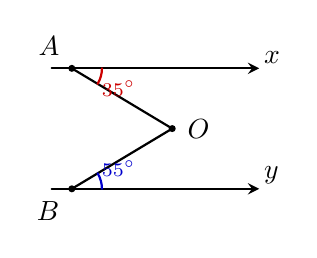
\begin{tikzpicture}[scale=0.85, >=stealth, line join=round, line cap=round]
  % Hai tia Ax va By
  \draw[thick, ->] (0.5, 2.3) -- (3.6, 2.3) node[above right=-2pt] {$x$};
  \draw[thick, ->] (0.5, 0.5) -- (3.6, 0.5) node[above right=-2pt] {$y$};
  
  % Doan AO va BO
  \draw[thick] (0.8, 2.3) -- (2.3, 1.4) -- (0.8, 0.5);
  
  % Diem A, B, O
  \fill (0.8, 2.3) circle (1.5pt) node[above left=1pt] {$A$};
  \fill (0.8, 0.5) circle (1.5pt) node[below left=1pt] {$B$};
  \fill (2.3, 1.4) circle (1.5pt) node[right=2pt] {$O$};
  
  % Goc xAO va yBO
  \draw[red!80!black, thick] (0.8, 2.3) ++(0:0.45) arc (0:-31:0.45);
  \node[red!80!black, font=\scriptsize] at (1.5, 2.0) {$35^\circ$};
  
  \draw[blue!80!black, thick] (0.8, 0.5) ++(0:0.45) arc (0:31:0.45);
  \node[blue!80!black, font=\scriptsize] at (1.5, 0.8) {$55^\circ$};
\end{tikzpicture}
\end{minipage}\par
\vspace{0.4mm}
\noindent\textit{Bài giải:}\dongkeHaiCot{10}
\\ \hline
\end{tabularx}

\vspace{1.5mm}

\noindent
\begin{tabularx}{\linewidth}{|X|}
\hline
\vspace{0.5mm}
\textbf{Câu 14 (0,5 điểm).} Tìm giá trị nhỏ nhất của biểu thức: $A = |x - 2025| + |x - 1|$.\par
\vspace{0.4mm}
\noindent\textit{Bài giải:}\dongkeHaiCot{6}
\\ \hline
\end{tabularx}

\newpage
% =============================================================================
% ========================= TOÁN 7 - TUẦN 08 - BUỔI 01: MÃ ĐỀ 103 =============
% ========================= MẶT TRƯỚC (TRANG 1/2) ==============================
% =============================================================================

\noindent
\begin{tabularx}{\linewidth}{|X|c|}
\hline
\textbf{PHIẾU KIỂM TRA ĐỊNH KỲ TOÁN 7 - TUẦN 08 - BUỔI 01} & \textbf{Mã đề: 103 - Trang 1/2} \\
\hline
\end{tabularx}

\vspace{1.2mm}

\noindent
\begin{tabularx}{\linewidth}{|p{3.2cm}|X|}
\hline
\centering\textbf{ĐIỂM SỐ} & \centering\textbf{LỜI NHẬN XÉT CỦA THẦY CÔ} \tabularnewline
\hline
\rule{0pt}{1.8cm} & \tabularnewline
\hline
\end{tabularx}

\vspace{1.5mm}

\noindent\textbf{Câu 1 (0,25 điểm).} Số đối của số hữu tỉ $-\frac{9}{16}$ là: \shortans{\frac{9}{16}}\par\vspace{2.4mm}
\noindent\textbf{Câu 2 (0,25 điểm).} Giá trị của biểu thức $\sqrt{\frac{81}{121}}$ bằng: \shortans{\frac{9}{11}}\par\vspace{2.4mm}
\noindent\textbf{Câu 3 (0,25 điểm).} Giá trị của biểu thức $|-6{,}8| + |3{,}2|$ bằng: \shortans{10}\par\vspace{2.4mm}
\noindent\textbf{Câu 4 (0,25 điểm).} Làm tròn số thập phân $37{,}584$ đến hàng phần mười: \shortans{37{,}6}\par\vspace{2.4mm}
\noindent\textbf{Câu 5 (0,25 điểm).} Hai đường thẳng cắt nhau tạo góc $75^\circ$. Góc đối đỉnh với nó có số đo là: \shortans{75^\circ}\par\vspace{2.4mm}
\noindent\textbf{Câu 6 (0,25 điểm).} Cho hai góc kề bù $\widehat{xOy}$ và $\widehat{yOz}$, biết $\widehat{xOy} = 50^\circ$. Số đo $\widehat{yOz}$ là: \shortans{130^\circ}\par\vspace{2.4mm}
\noindent\textbf{Câu 7 (0,25 điểm).} Tia $Ot$ là tia phân giác của góc $\widehat{xOy} = 140^\circ$. Số đo của $\widehat{xOt}$ là: \shortans{70^\circ}\par\vspace{2.4mm}
\noindent\textbf{Câu 8 (0,25 điểm).} Cho $a \parallel b$. Một góc trong cùng phía với góc $70^\circ$ có số đo là: \shortans{110^\circ}\par\vspace{2.4mm}
\noindent\textbf{Câu 9 (0,25 điểm).} Hai đường thẳng phân biệt cùng song song với đường thẳng thứ ba thì hai đường thẳng đó: \shortans{\text{song song}}\par\vspace{2.4mm}
\noindent\textbf{Câu 10 (0,25 điểm).} Một đôi giày giá $300\,000$ đồng, đang giảm giá $15\%$. Số tiền được giảm là: \shortans{45\,000\text{ đ}}\par\vspace{2.4mm}
\vspace{0.4mm}

\noindent\textbf{Câu 11 (3,0 điểm). Thực hiện phép tính (hợp lý nếu có thể):}
\vspace{0.8mm}

\noindent
\begin{tabularx}{\linewidth}{|X|X|}
\hline
\oBaiTap[5]{a) (0,5 điểm)}{$\dfrac{9}{17} - \dfrac{4}{9} + \dfrac{8}{17} - \dfrac{5}{9}$} & 
\oBaiTap[5]{b) (0,5 điểm)}{$\dfrac{17}{21} \cdot \dfrac{3}{8} + \dfrac{17}{21} \cdot \dfrac{5}{8} - \dfrac{17}{21}$} \\
\hline
\oBaiTap[5]{c) (0,5 điểm)}{$\left(-\dfrac{1}{2}\right)^4 \cdot 32 + \left(-\dfrac{2}{3}\right)^2 \cdot 18$} & 
\oBaiTap[5]{d) (0,5 điểm)}{$\sqrt{\dfrac{64}{9}} - \left|-\dfrac{5}{3}\right| + \sqrt{100}$} \\
\hline
\oBaiTap[5]{e) (0,5 điểm)}{$\left(\dfrac{2}{3} - 0{,}25\right) : \dfrac{5}{12} + \dfrac{4}{7} \cdot 1{,}4$} & 
\oBaiTap[5]{f) (0,5 điểm)}{$\dfrac{4^3 \cdot 9^2}{6^4}$} \\
\hline
\end{tabularx}

\newpage
% =============================================================================
% ========================= TOÁN 7 - TUẦN 08 - BUỔI 01: MÃ ĐỀ 103 =============
% ========================= MẶT SAU (TRANG 2/2) ================================
% =============================================================================

\noindent
\begin{tabularx}{\linewidth}{|X|c|}
\hline
\textbf{TOÁN 7 - TUẦN 08 - BUỔI 01} & \textbf{Mã đề: 103 - Trang 2/2} \\
\hline
\end{tabularx}

\vspace{1.5mm}

\noindent\textbf{Câu 12 (2,0 điểm). Tìm số hữu tỉ $x$, biết:}
\vspace{0.8mm}

\noindent
\begin{tabularx}{\linewidth}{|X|X|}
\hline
\oBaiTap[5]{a) (0,5 điểm)}{$x + \dfrac{3}{4} = \dfrac{11}{12}$} & 
\oBaiTap[5]{b) (0,5 điểm)}{$\dfrac{4}{5}x - \dfrac{1}{2} = \dfrac{11}{10}$} \\
\hline
\oBaiTap[5]{c) (0,5 điểm)}{$\left(x - \dfrac{1}{4}\right)^2 = \dfrac{25}{36}$} & 
\oBaiTap[5]{d) (0,5 điểm)}{$\left|3x - \dfrac{1}{4}\right| = \dfrac{11}{4}$} \\
\hline
\end{tabularx}

\vspace{1.5mm}

\noindent
\begin{tabularx}{\linewidth}{|X|}
\hline
\vspace{0.5mm}
\begin{minipage}[t]{0.68\linewidth}
\vspace{0pt}
\textbf{Câu 13 (2,0 điểm).} Cho hai tia $Ax$ và $By$ song song với nhau ($Ax \parallel By$). Điểm $O$ nằm giữa hai đường thẳng chứa tia $Ax$ và $By$ sao cho tia $Ax$ và tia $By$ cùng nằm về một phía đối với đường thẳng $AB$. Biết $\widehat{xAO} = 45^\circ$ và $\widehat{yBO} = 65^\circ$.\par\vspace{0.4mm}
\textbf{a) (1,0 điểm)} Kẻ tia $Oz \parallel Ax$ (tia $Oz$ nằm trong góc $\widehat{AOB}$). Giải thích vì sao $Oz \parallel By$.\par\vspace{0.4mm}
\textbf{b) (1,0 điểm)} Tính số đo góc $\widehat{AOB}$.
\end{minipage}\hfill
\begin{minipage}[t]{0.30\linewidth}
\vspace{0pt}\centering
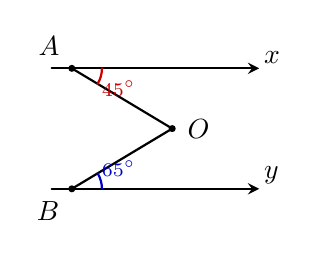
\begin{tikzpicture}[scale=0.85, >=stealth, line join=round, line cap=round]
  % Hai tia Ax va By
  \draw[thick, ->] (0.5, 2.3) -- (3.6, 2.3) node[above right=-2pt] {$x$};
  \draw[thick, ->] (0.5, 0.5) -- (3.6, 0.5) node[above right=-2pt] {$y$};
  
  % Doan AO va BO
  \draw[thick] (0.8, 2.3) -- (2.3, 1.4) -- (0.8, 0.5);
  
  % Diem A, B, O
  \fill (0.8, 2.3) circle (1.5pt) node[above left=1pt] {$A$};
  \fill (0.8, 0.5) circle (1.5pt) node[below left=1pt] {$B$};
  \fill (2.3, 1.4) circle (1.5pt) node[right=2pt] {$O$};
  
  % Goc xAO va yBO
  \draw[red!80!black, thick] (0.8, 2.3) ++(0:0.45) arc (0:-31:0.45);
  \node[red!80!black, font=\scriptsize] at (1.5, 2.0) {$45^\circ$};
  
  \draw[blue!80!black, thick] (0.8, 0.5) ++(0:0.45) arc (0:31:0.45);
  \node[blue!80!black, font=\scriptsize] at (1.5, 0.8) {$65^\circ$};
\end{tikzpicture}
\end{minipage}\par
\vspace{0.4mm}
\noindent\textit{Bài giải:}\dongkeHaiCot{10}
\\ \hline
\end{tabularx}

\vspace{1.5mm}

\noindent
\begin{tabularx}{\linewidth}{|X|}
\hline
\vspace{0.5mm}
\textbf{Câu 14 (0,5 điểm).} Tìm giá trị nhỏ nhất của biểu thức: $A = |x - 2026| + |x - 6|$.\par
\vspace{0.4mm}
\noindent\textit{Bài giải:}\dongkeHaiCot{6}
\\ \hline
\end{tabularx}

\newpage
% =============================================================================
% ========================= TOÁN 7 - TUẦN 08 - BUỔI 01: MÃ ĐỀ 104 =============
% ========================= MẶT TRƯỚC (TRANG 1/2) ==============================
% =============================================================================

\noindent
\begin{tabularx}{\linewidth}{|X|c|}
\hline
\textbf{PHIẾU KIỂM TRA ĐỊNH KỲ TOÁN 7 - TUẦN 08 - BUỔI 01} & \textbf{Mã đề: 104 - Trang 1/2} \\
\hline
\end{tabularx}

\vspace{1.2mm}

\noindent
\begin{tabularx}{\linewidth}{|p{3.2cm}|X|}
\hline
\centering\textbf{ĐIỂM SỐ} & \centering\textbf{LỜI NHẬN XÉT CỦA THẦY CÔ} \tabularnewline
\hline
\rule{0pt}{1.8cm} & \tabularnewline
\hline
\end{tabularx}

\vspace{1.5mm}

\noindent\textbf{Câu 1 (0,25 điểm).} Số đối của số hữu tỉ $-\frac{11}{20}$ là: \shortans{\frac{11}{20}}\par\vspace{2.4mm}
\noindent\textbf{Câu 2 (0,25 điểm).} Giá trị của biểu thức $\sqrt{\frac{121}{144}}$ bằng: \shortans{\frac{11}{12}}\par\vspace{2.4mm}
\noindent\textbf{Câu 3 (0,25 điểm).} Giá trị của biểu thức $|-7{,}5| + |3{,}5|$ bằng: \shortans{11}\par\vspace{2.4mm}
\noindent\textbf{Câu 4 (0,25 điểm).} Làm tròn số thập phân $46{,}293$ đến hàng phần mười: \shortans{46{,}3}\par\vspace{2.4mm}
\noindent\textbf{Câu 5 (0,25 điểm).} Hai đường thẳng cắt nhau tạo góc $85^\circ$. Góc đối đỉnh với nó có số đo là: \shortans{85^\circ}\par\vspace{2.4mm}
\noindent\textbf{Câu 6 (0,25 điểm).} Cho hai góc kề bù $\widehat{xOy}$ và $\widehat{yOz}$, biết $\widehat{xOy} = 80^\circ$. Số đo $\widehat{yOz}$ là: \shortans{100^\circ}\par\vspace{2.4mm}
\noindent\textbf{Câu 7 (0,25 điểm).} Tia $Ot$ là tia phân giác của góc $\widehat{xOy} = 160^\circ$. Số đo của $\widehat{xOt}$ là: \shortans{80^\circ}\par\vspace{2.4mm}
\noindent\textbf{Câu 8 (0,25 điểm).} Cho $a \parallel b$. Một góc trong cùng phía với góc $80^\circ$ có số đo là: \shortans{100^\circ}\par\vspace{2.4mm}
\noindent\textbf{Câu 9 (0,25 điểm).} Hai đường thẳng phân biệt cùng vuông góc với đường thẳng thứ ba thì hai đường thẳng đó: \shortans{\text{song song}}\par\vspace{2.4mm}
\noindent\textbf{Câu 10 (0,25 điểm).} Một chiếc áo khoác giá $400\,000$ đồng, đang giảm giá $10\%$. Số tiền được giảm là: \shortans{40\,000\text{ đ}}\par\vspace{2.4mm}
\vspace{0.4mm}

\noindent\textbf{Câu 11 (3,0 điểm). Thực hiện phép tính (hợp lý nếu có thể):}
\vspace{0.8mm}

\noindent
\begin{tabularx}{\linewidth}{|X|X|}
\hline
\oBaiTap[5]{a) (0,5 điểm)}{$\dfrac{6}{19} - \dfrac{5}{11} + \dfrac{13}{19} - \dfrac{6}{11}$} & 
\oBaiTap[5]{b) (0,5 điểm)}{$\dfrac{14}{25} \cdot \dfrac{7}{10} + \dfrac{14}{25} \cdot \dfrac{3}{10} - \dfrac{14}{25}$} \\
\hline
\oBaiTap[5]{c) (0,5 điểm)}{$\left(-\dfrac{3}{2}\right)^2 \cdot 8 - \left(-\dfrac{1}{3}\right)^3 \cdot 54$} & 
\oBaiTap[5]{d) (0,5 điểm)}{$\sqrt{\dfrac{121}{36}} - \left|-\dfrac{5}{6}\right| + \sqrt{121}$} \\
\hline
\oBaiTap[5]{e) (0,5 điểm)}{$\left(\dfrac{3}{5} - 0{,}25\right) : \dfrac{7}{20} + \dfrac{5}{9} \cdot 1{,}8$} & 
\oBaiTap[5]{f) (0,5 điểm)}{$\dfrac{25^2 \cdot 4^3}{10^4}$} \\
\hline
\end{tabularx}

\newpage
% =============================================================================
% ========================= TOÁN 7 - TUẦN 08 - BUỔI 01: MÃ ĐỀ 104 =============
% ========================= MẶT SAU (TRANG 2/2) ================================
% =============================================================================

\noindent
\begin{tabularx}{\linewidth}{|X|c|}
\hline
\textbf{TOÁN 7 - TUẦN 08 - BUỔI 01} & \textbf{Mã đề: 104 - Trang 2/2} \\
\hline
\end{tabularx}

\vspace{1.5mm}

\noindent\textbf{Câu 12 (2,0 điểm). Tìm số hữu tỉ $x$, biết:}
\vspace{0.8mm}

\noindent
\begin{tabularx}{\linewidth}{|X|X|}
\hline
\oBaiTap[5]{a) (0,5 điểm)}{$x + \dfrac{2}{7} = \dfrac{11}{14}$} & 
\oBaiTap[5]{b) (0,5 điểm)}{$\dfrac{5}{6}x - \dfrac{1}{4} = \dfrac{17}{12}$} \\
\hline
\oBaiTap[5]{c) (0,5 điểm)}{$\left(x - \dfrac{1}{5}\right)^2 = \dfrac{9}{25}$} & 
\oBaiTap[5]{d) (0,5 điểm)}{$\left|2x - \dfrac{1}{5}\right| = \dfrac{9}{5}$} \\
\hline
\end{tabularx}

\vspace{1.5mm}

\noindent
\begin{tabularx}{\linewidth}{|X|}
\hline
\vspace{0.5mm}
\begin{minipage}[t]{0.68\linewidth}
\vspace{0pt}
\textbf{Câu 13 (2,0 điểm).} Cho hai tia $Ax$ và $By$ song song với nhau ($Ax \parallel By$). Điểm $O$ nằm giữa hai đường thẳng chứa tia $Ax$ và $By$ sao cho tia $Ax$ và tia $By$ cùng nằm về một phía đối với đường thẳng $AB$. Biết $\widehat{xAO} = 50^\circ$ và $\widehat{yBO} = 60^\circ$.\par\vspace{0.4mm}
\textbf{a) (1,0 điểm)} Kẻ tia $Oz \parallel Ax$ (tia $Oz$ nằm trong góc $\widehat{AOB}$). Giải thích vì sao $Oz \parallel By$.\par\vspace{0.4mm}
\textbf{b) (1,0 điểm)} Tính số đo góc $\widehat{AOB}$.
\end{minipage}\hfill
\begin{minipage}[t]{0.30\linewidth}
\vspace{0pt}\centering
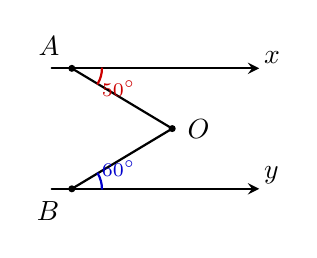
\begin{tikzpicture}[scale=0.85, >=stealth, line join=round, line cap=round]
  % Hai tia Ax va By
  \draw[thick, ->] (0.5, 2.3) -- (3.6, 2.3) node[above right=-2pt] {$x$};
  \draw[thick, ->] (0.5, 0.5) -- (3.6, 0.5) node[above right=-2pt] {$y$};
  
  % Doan AO va BO
  \draw[thick] (0.8, 2.3) -- (2.3, 1.4) -- (0.8, 0.5);
  
  % Diem A, B, O
  \fill (0.8, 2.3) circle (1.5pt) node[above left=1pt] {$A$};
  \fill (0.8, 0.5) circle (1.5pt) node[below left=1pt] {$B$};
  \fill (2.3, 1.4) circle (1.5pt) node[right=2pt] {$O$};
  
  % Goc xAO va yBO
  \draw[red!80!black, thick] (0.8, 2.3) ++(0:0.45) arc (0:-31:0.45);
  \node[red!80!black, font=\scriptsize] at (1.5, 2.0) {$50^\circ$};
  
  \draw[blue!80!black, thick] (0.8, 0.5) ++(0:0.45) arc (0:31:0.45);
  \node[blue!80!black, font=\scriptsize] at (1.5, 0.8) {$60^\circ$};
\end{tikzpicture}
\end{minipage}\par
\vspace{0.4mm}
\noindent\textit{Bài giải:}\dongkeHaiCot{10}
\\ \hline
\end{tabularx}

\vspace{1.5mm}

\noindent
\begin{tabularx}{\linewidth}{|X|}
\hline
\vspace{0.5mm}
\textbf{Câu 14 (0,5 điểm).} Tìm giá trị nhỏ nhất của biểu thức: $A = |x - 2024| + |x - 4|$.\par
\vspace{0.4mm}
\noindent\textit{Bài giải:}\dongkeHaiCot{6}
\\ \hline
\end{tabularx}

\newpage
\end{document}